\chapter{Chapter 5 Supplemental Information}
\label{sec:app5}
\clearpage
\section{Supplemental Figures}


%Supplemental Figure 8: Shifts in CORE

\begin{figure}[h!]

  \centering
  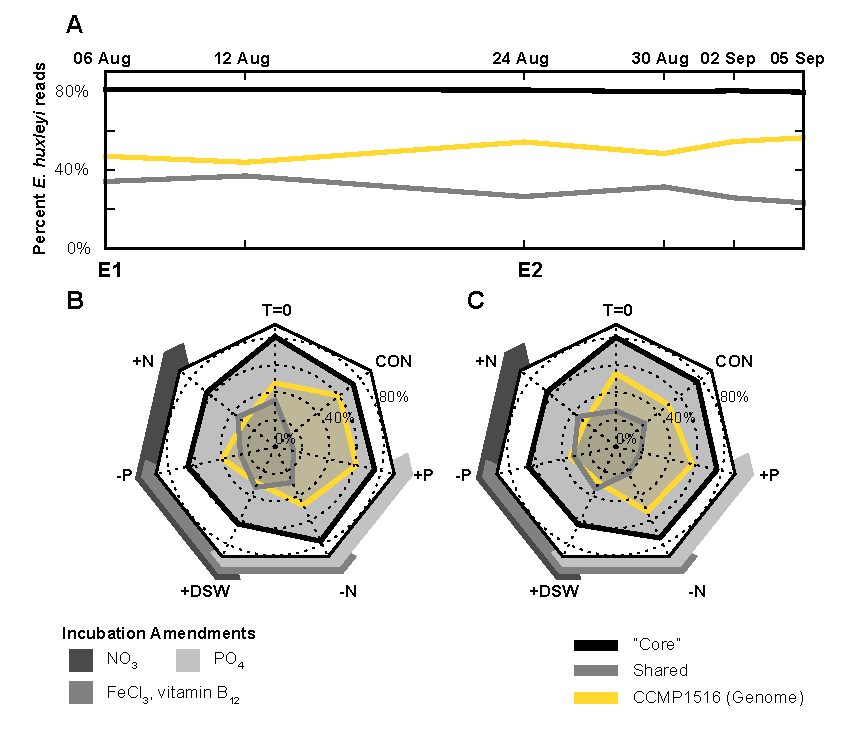
\includegraphics[width=1\textwidth]{Images/C6_FigureS8_core_genes.pdf}
  \caption[The relative expression of `core', shared, and CCMP1516-specific transcripts across time and in incubation experiments]{The relative expression of `core', shared, and CCMP1516-specific transcripts across time and in incubation experiments. The percentage of all mapped reads corresponding to the genes considered to be `core' by Read et al. (2013) (black), found to be shared across the five strains used in this study (grey), or originally considered to be unique to CCMP1516 are plotted for each \textit{in situ} sample (A) and in each of the two replicated incubation experiments, E1 (B) and E2 (C). Nutrients added to incubation experiments are indicated on the exterior of the radar plots, indicating the addition of nitrate, phosphate, trace metals, and vitamins.}
    \label{fig:a5f8}
\end{figure}




%Supplemental Figure 1: Nutrient concentrations at Tf

\begin{figure}[h!]
  \centering
    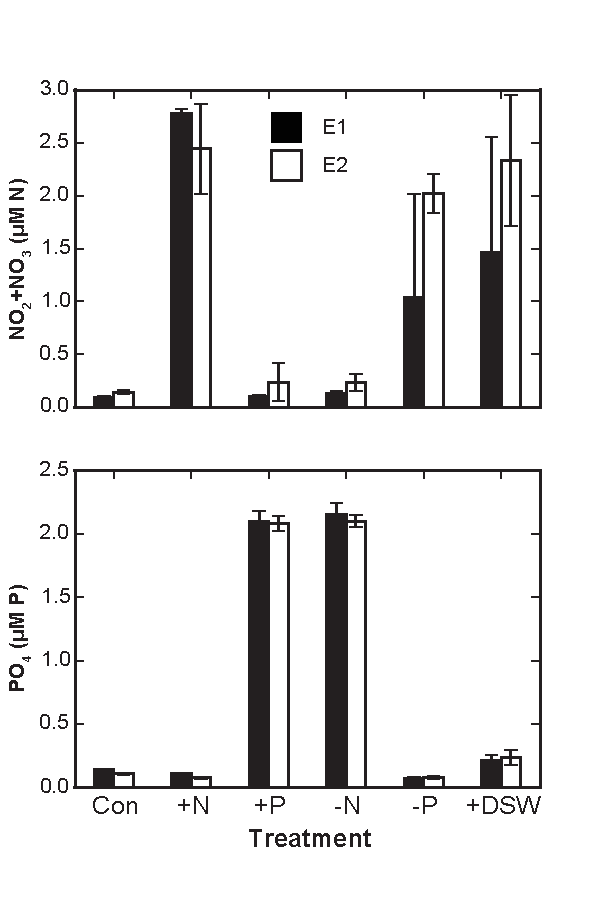
\includegraphics[width=.6\textwidth]{Images/C6_FigureS1_nutrients_v1.pdf}
    \caption{Inorganic nitrogen and phosphorus concentrations at the point of RNA sampling (7 days post-inoculation) for each of the six treatments in E1 and E2, averaged across triplicate bottles (n=3).}
    \label{fig:a5f1}
\end{figure}


%Supplemental Figure 2: KOG distributions across genes

\begin{figure}[p!]
  \centering
    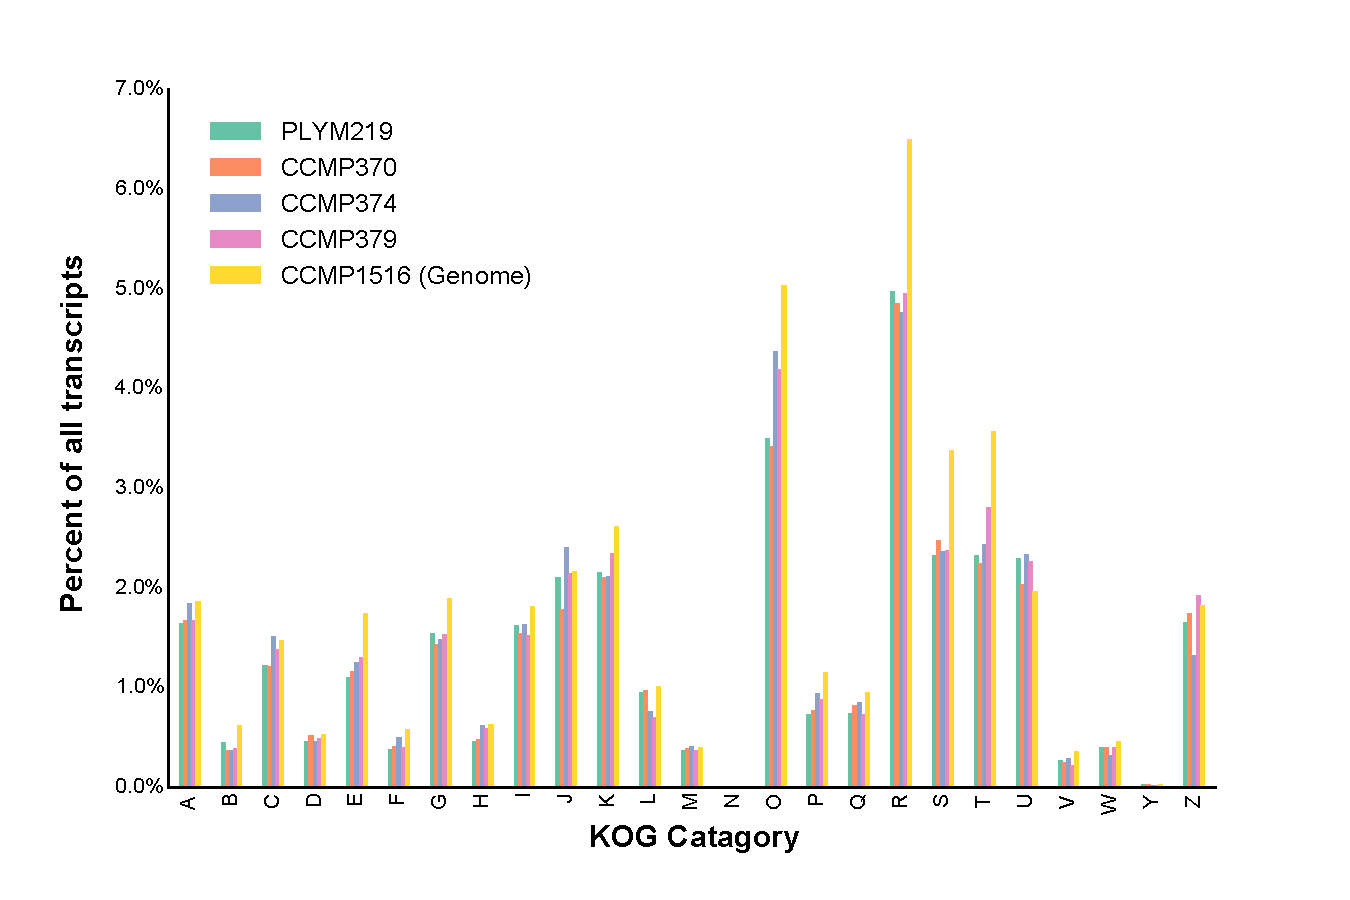
\includegraphics[width=1.0\textwidth]{Images/C6_FigureS2_KOG_Distribution}
    \caption{The percent of genes falling into each of the KOG classes for each of the five strains.}
    \label{fig:a5f2}
\end{figure}

%Supplemental Figure 3: Distributions across genes

\begin{figure}[p!]
  \centering
    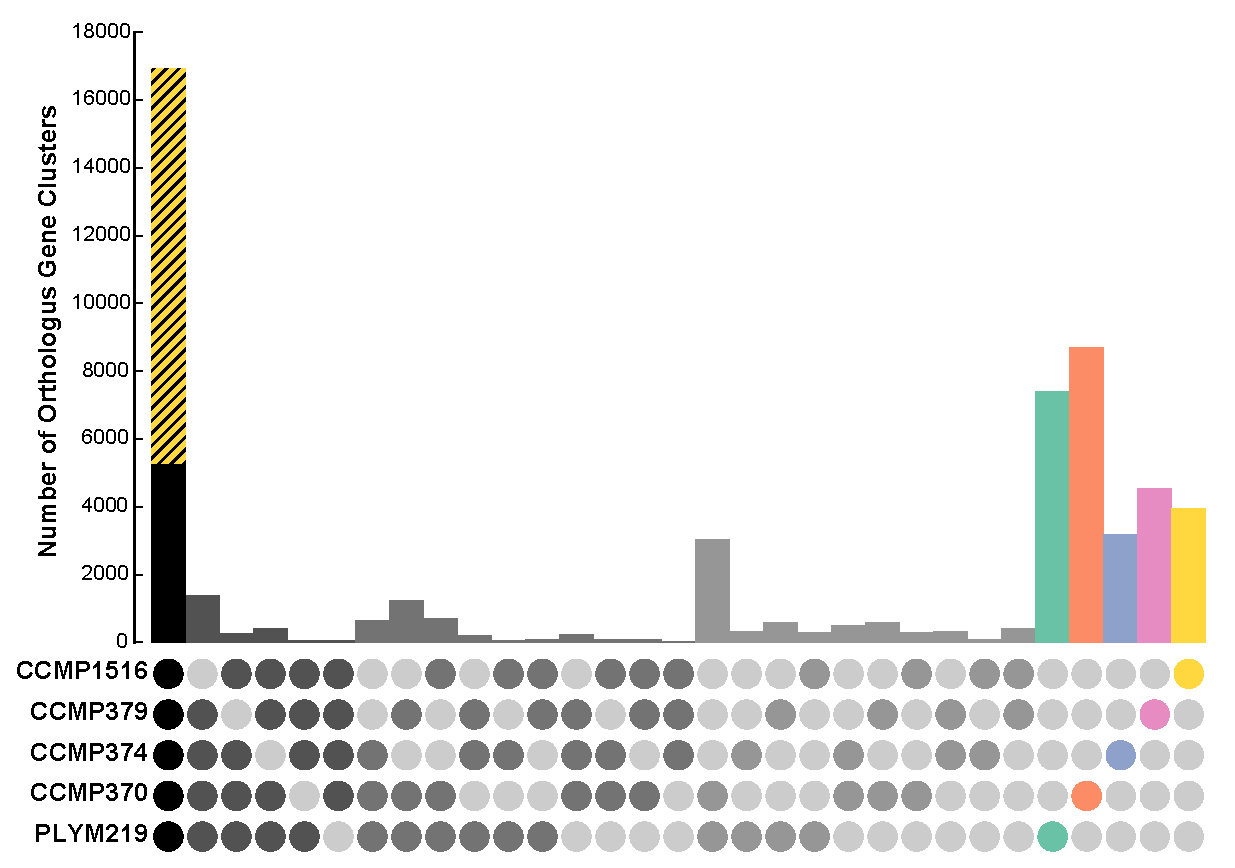
\includegraphics[width=1.0\textwidth]{Images/C6_FigureS3_GeneDistrubtion.pdf}
    \caption[The number of orthologous groups falling into each of the possible strain sets across the five strains surveyed]{The number of orthologous groups falling into each of the possible strain sets across the five strains surveyed. The relative strain membership is depicted in a scatter plot along the x-axis ranging from the first row of 'shared' or `core' genes, common to all strains (black), through variable memberships across some but not all strains, to sets comprised of only one strain (colored). Genes common to all strains in this study are shown in black. Genes identified as `core' in CCMP1516, the genome strain, by Read et al. (2013), but that were not identified in some or all of the other strains were added to the `shared' set and are indicated in yellow hatching. }
    \label{fig:a5f3}
\end{figure}


%Supplemental Figure 4: MANTA

\begin{figure}[p!]
  \centering
    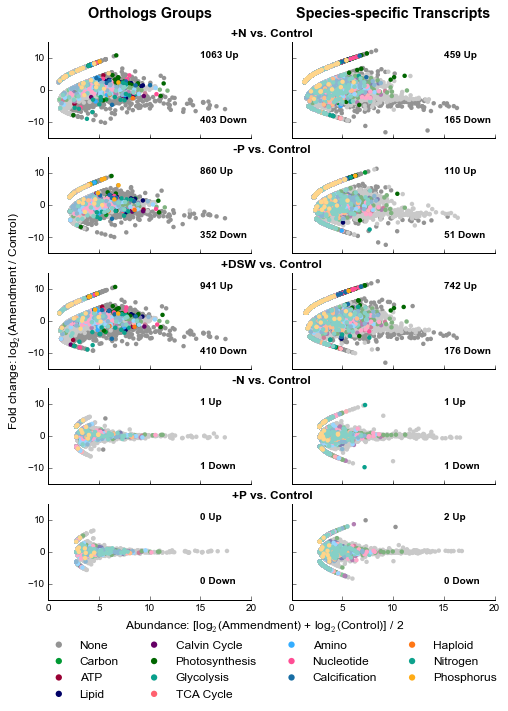
\includegraphics[width=0.8\textwidth]{Images/C6_FigureS4_MANTA.png}
    \caption[Log normalized fold change plotted against log normalized average abundance for each of the five amended treatments compared to the no-addition control]{Log normalized fold change plotted against log normalized average abundance for each of the five amended treatments compared to the no-addition control. edgeR was used to assess the average abundance and log fold change for each of the orthologous groups (left column) and strain-specific transcripts (right column). Genes are colored by generalized metabolic function. The intensity of the color indicates significance, with opaque indicating significance (FDR < 0.05). }
    \label{fig:a5f4}
\end{figure}


%Supplemental Figure 5: Venn 

\begin{figure}[p!]
  \centering
    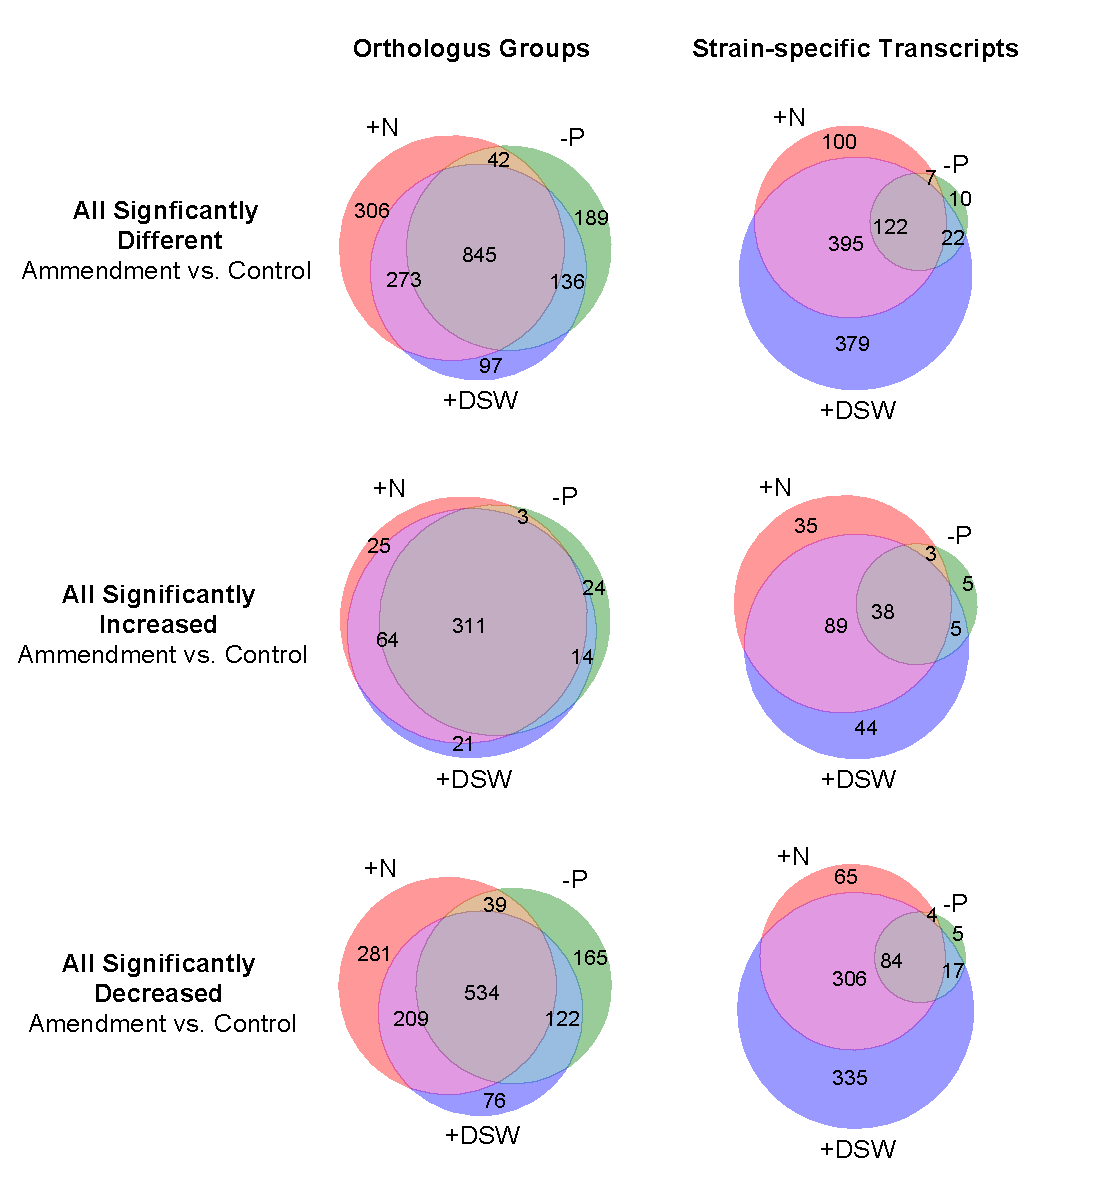
\includegraphics[width=0.8\textwidth]{Images/C6_FigureS5_Venn_DEGenes.pdf}
    \caption[Weighted Venn diagrams of significantly different, increased, and decreased orthologus groups and species-specific transcripts across each of the amendedments to which N was added. ]{Weighted Venn diagrams of significantly (FDR $< 0.05$) different, increased, and decreased orthologus groups and species-specific transcripts across each of the amendments to which N was added (+N, -P, +DSW).}
    \label{fig:a5f5}
\end{figure}

%Supplemental Figure 6: Carbon, Nucleotide etc. 


\begin{figure}[p!]

  \centering
  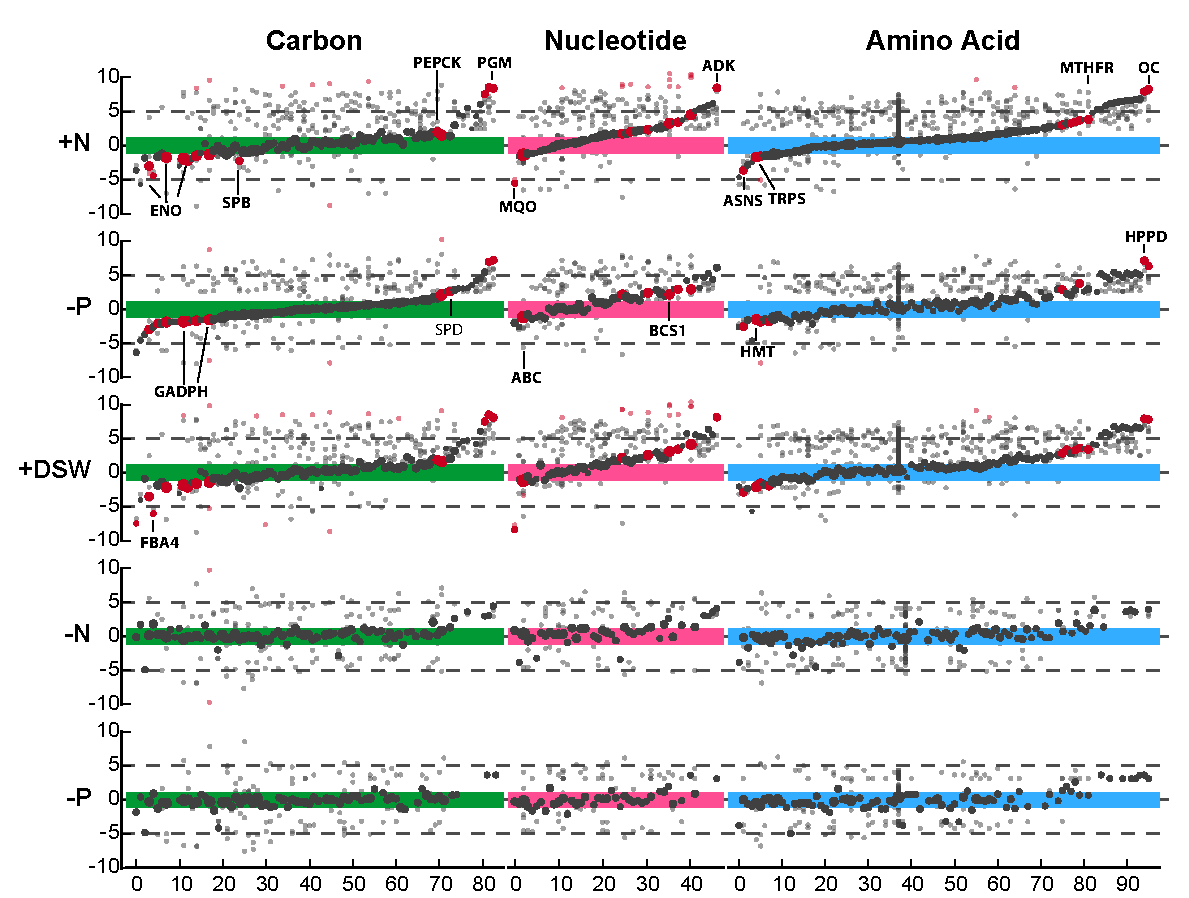
\includegraphics[width=1\textwidth]{Images/C6_FigureS6_MckewCarbon.pdf}
    \caption[Fold change of genes associated with carbon, nucleotide, and amino acid metabolism across each of the incubation amendments]{Fold change of genes associated with carbon, nucleotide, and amino acid metabolism across each of the incubation amendments compared to the no addition control. The log fold change of orthologous groups associated with carbon, nucleotide, and amino acid metabolism was assessed with edgeR across the five amended incubations compared to the no addition control are plotted in opaque grey. The size of the orthologous group marker is proportionate to the log of the mean abundance across the two treatments. Orthologous groups are that are significantly differentially abundant (FDR < 0.05) are plotted highlighted in red. Individual transcripts within an orthologous group are plotted in light grey or red to indicate significance of fold change. Genes of interest are labeled with abbreviations as follows, labels in bold indicate significant regulation in two or more conditions. }
    \label{fig:a5f6}
\end{figure}

%Supplemental Figure 7: ATP

\begin{figure}[p!]

  \centering
  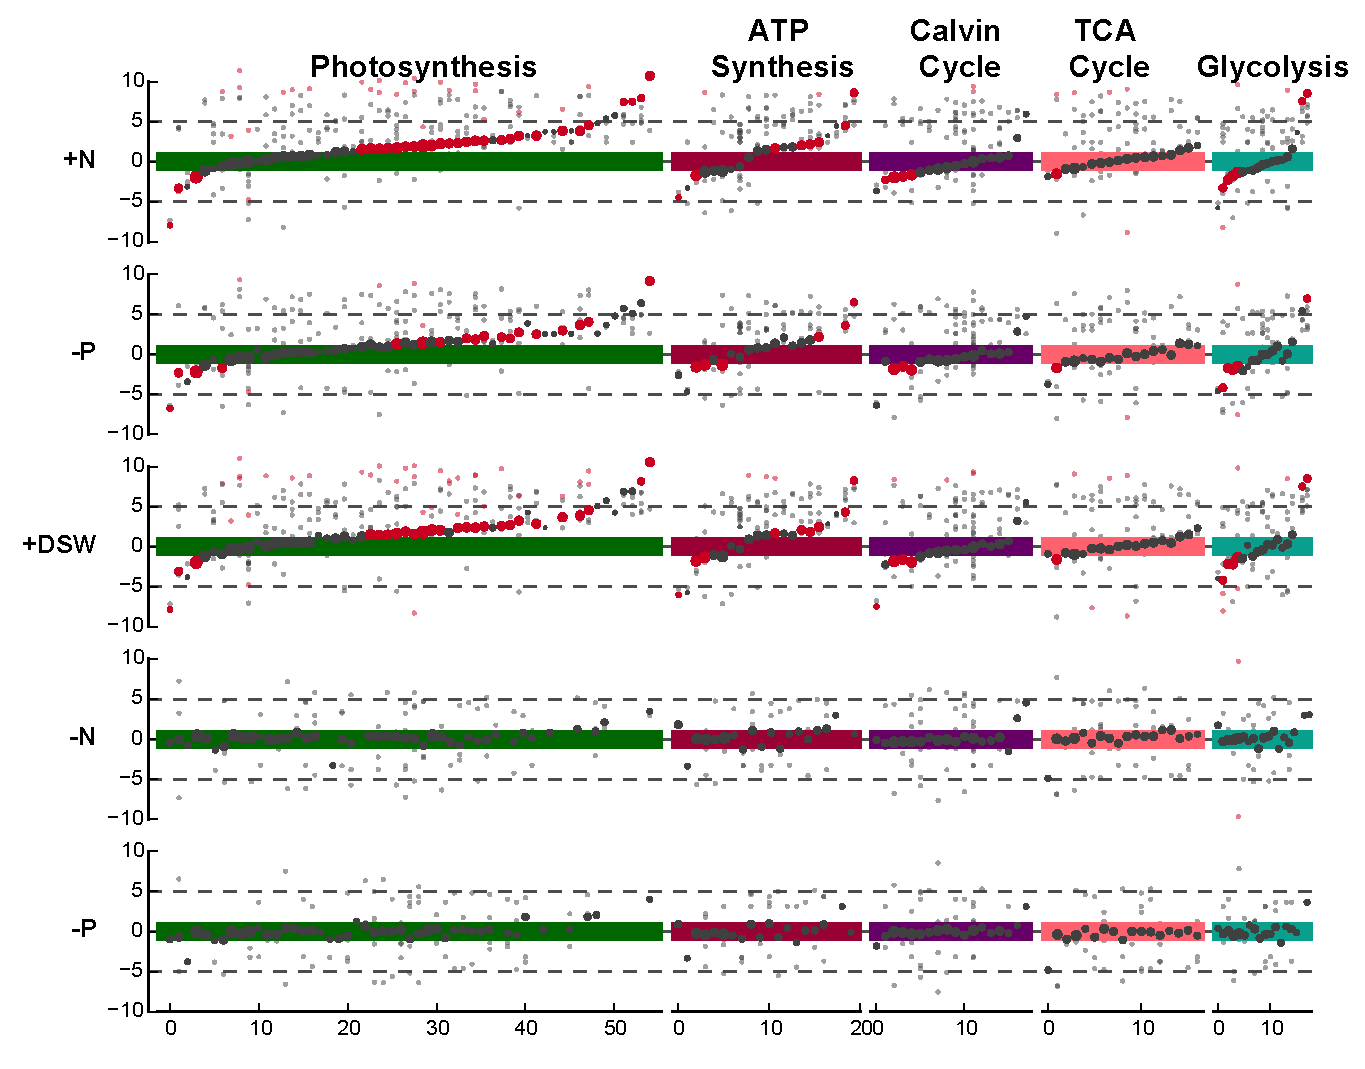
\includegraphics[width=1\textwidth]{Images/C6_FigureS7_MckewATP.pdf}
    \caption[Fold change of genes associated with photosynthesis, ATP synthesis, Calvin cycle, TCA cycle, and glycolysis across each of the incubation amendments]{Fold change of genes associated with photosynthesis, ATP synthesis, Calvin cycle, TCA cycle, and glycolysis across each of the incubation amendments compared to the no addition control. The log fold change of orthologous groups associated with photosynthesis, ATP synthesis, Calvin cycle, TCA cycle, and glycolysis was assessed with edgeR across the five amended incubations compared to the no addition control are plotted in opaque grey. The size of the orthologous group marker is proportionate to the log of the mean abundance across the two treatments. Orthologous groups are that are significantly differentially abundant (FDR < 0.05) are plotted highlighted in red. Individual transcripts within an orthologous group are plotted in light grey or red to indicate significance of fold change. Genes of interest are labeled with abbreviations as follows, labels in bold indicate significant regulation in two or more conditions. }
    \label{fig:a5f7}
\end{figure}



%Supplemental Figure 9: Annotation of Core

\begin{figure}[p!]

  \centering
  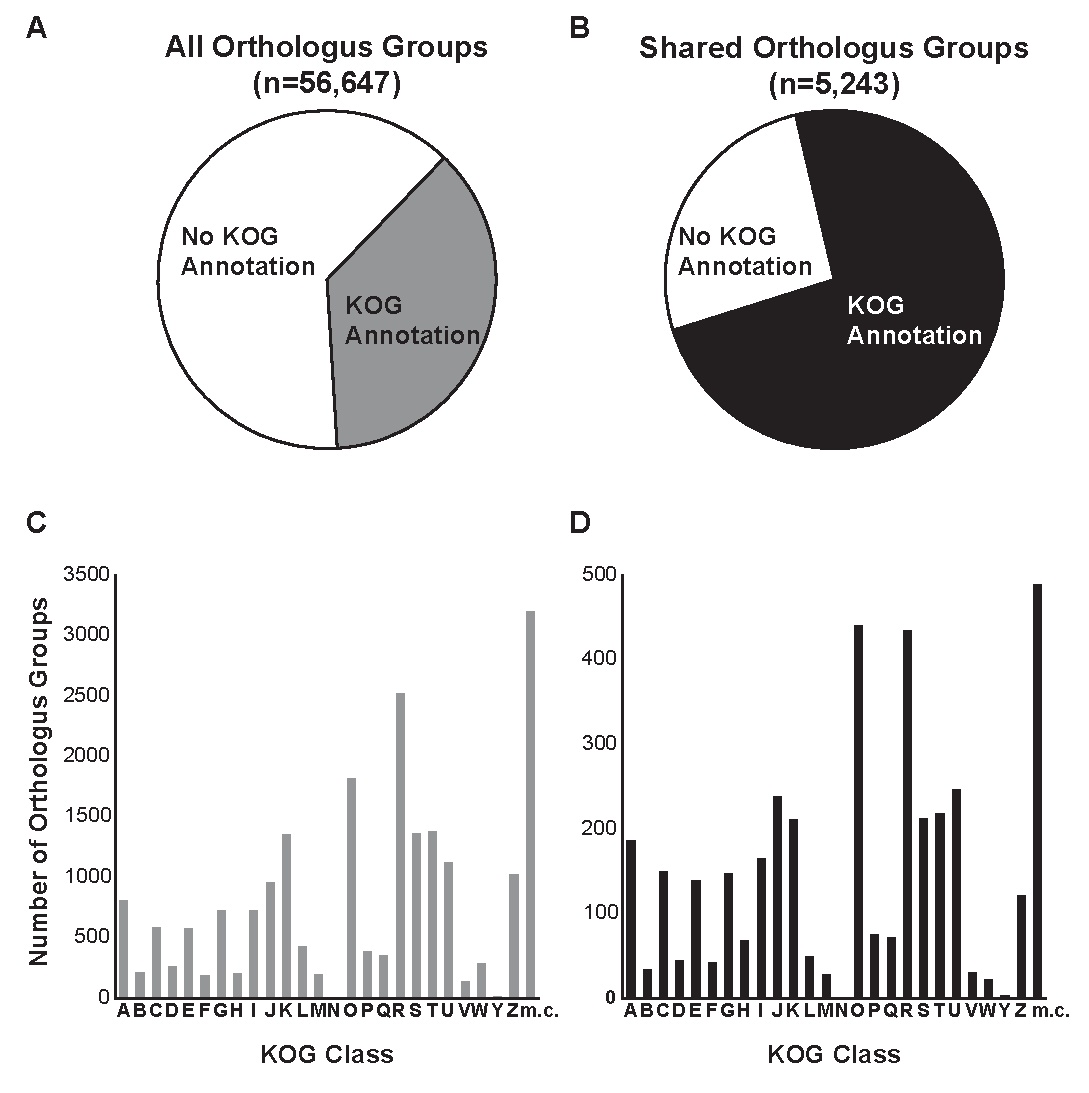
\includegraphics[width=.75\textwidth]{Images/C6_FigureS9_KOGAnnotation.pdf}
  \caption[Annotation of orthologous groups using KOG orthology for all \textit{E. huxleyi} orthologous groups and for shared orthologous groups]{Annotation of orthologous groups using KOG orthology for all \textit{E. huxleyi} orthologous groups and for shared orthologous groups. The relative percentage of orthologous groups able to be annotated for all orthologous groups (A) and orthologous group shared amongst the five studied strains (B) are shown. The number of orthologous groups falling into each KOG class or multiple classes (m.c.) is shown for both all orthologous groups (C) and shared groups (D). }
    \label{fig:a5f9}
\end{figure}


%Supplemental Figure 10: Strain composition of the shared gene set in the field


\begin{figure}[p!]

  \centering
  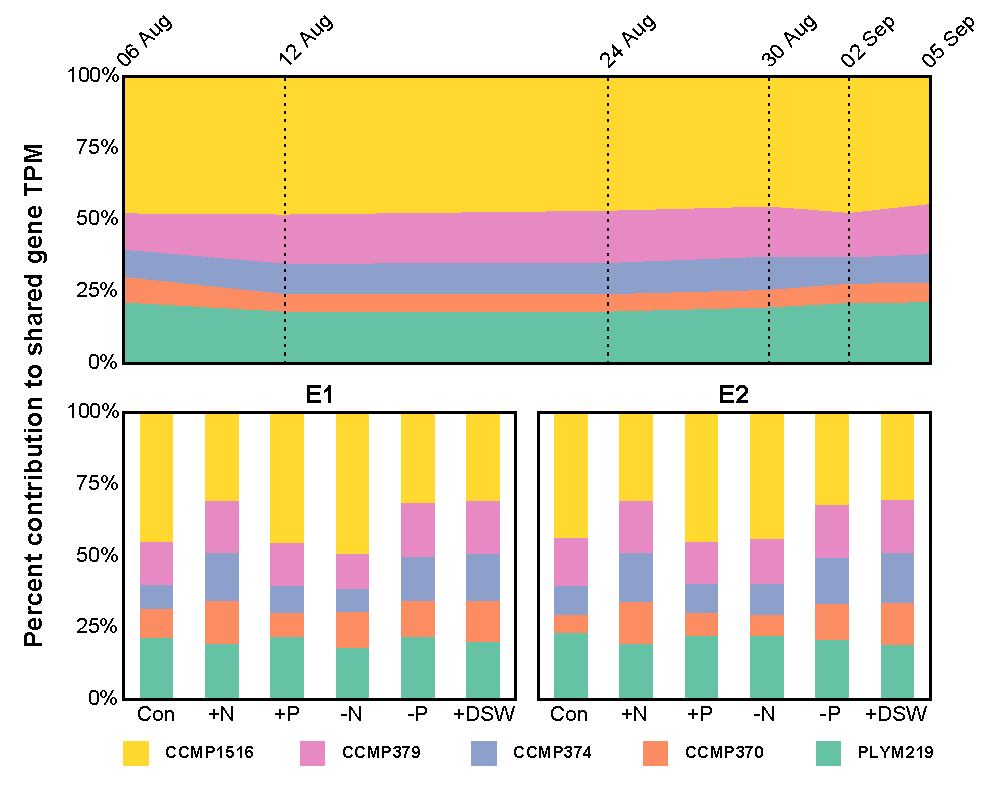
\includegraphics[width=1\textwidth]{Images/C6_FigureS10_SharedGeneComp.pdf}
  \caption[RSEM estimated contribution of each strain to the abundance of the shared set of genes in the field and incubation experiments]{RSEM estimated contribution of each strain to the abundance of the shared set of genes in the field and incubation experiments.}
    \label{fig:a5f10}
\end{figure}
\clearpage

\section{Supplemental Tables}

\begin{table}[h!]
\centering
\caption{Final nutrient concentrations used in nutrient amendment incubations.}
\label{tab:c5t1}
\small
\begin{tabular}{lllllll}
                              & \multicolumn{6}{c}{\textbf{Treatment}}                                                   \\ 
\textbf{Amendment}            & \textbf{Control} & \textbf{+N} & \textbf{+P} & \textbf{-N} & \textbf{-P} & \textbf{+DSW} \\ \Xhline{2\arrayrulewidth}
\textbf{Nitrate}              & -                & $4 \mu M$   & -           & -           & $4 \mu M$   & -             \\ 
\textbf{Phosphate}            & -                & -           & $3 \mu M$   & $3 \mu M$   & -           & -             \\ 
\textbf{Silica}               & -                & -           & -           & $8.7 \mu M$ & $8.7 \mu M$ & -             \\ 
\textbf{Iron}                 & -                & -           & -           & $5 nM$      & $5 nM$      & -             \\ 
\textbf{Vitamin B$_{12}$}     & -                & -           & -           & $100 pM$    & $100 pM$    & -             \\ 
\textbf{Deep Seawater (700m)} & -                & -           & -           & -           & -           & 10\% v/v      \\ 
\end{tabular}
\end{table}

\begin{landscape}
\begin{table}[h!]
\centering
\caption{Strain isolation date, synonyms, and transcriptome/genome information for each of the five strains used in this study.}
\label{tab:c5t2}
\small
\newcolumntype{L}[1]{>{\raggedright\let\newline\\\arraybackslash\hspace{0pt}}m{#1}}
\begin{tabular}{lL{1.25cm}L{2cm}L{2.5cm}L{2cm}L{2cm}L{2cm}L{3cm}L{3cm}}
\hline
\textbf{Strain}   & \textbf{Isolation date} & \textbf{Strain synonyms}                  & \textbf{Genome or Transcriptome} & \textbf{Predicted proteins} & \textbf{Transcripts passing quality control} & \textbf{Representative orthoMCL orthologus groups} & \textbf{MMETSP Sample IDs} & \textbf{Reference for genome/ transcriptome download}      \\ \Xhline{2\arrayrulewidth}

\textbf{CCMP1516} & 1991                    & CCMP2090                                  & Genome                           & 33341                                         & 32538                                        & 23792                                              & N/A                        & \href{http://genome.jgi.doe.gov/Emihu1/Emihu1.download.ftp.html}{JGI} \\ \hline
\textbf{CCMP370}  & 1959                    & 451B, F451                                & Transcriptome                    & 38712                                         & 33455                                        & 29068                                              & MMETSP1154-1157            & \href{http://data.imicrobe.us/combined\_assembly/view/34}{iMicrobe}        \\ \hline
\textbf{CCMP374}  & 1990                    & 89E, CCMP1949                             & Transcriptome                    & 18859                                         & 15728                                        & 14628                                              & MMETSP1006-1009            & \href{http://data.imicrobe.us/combined\_assembly/view/32}{iMicrobe}        \\ \hline
\textbf{CCMP379}  & 1957                    & 92A, P-92A, UTEX1061, CCAP/1A, Plymouth 2 & Transcriptome                    & 23300                                         & 20016                                        & 18561                                              & MMETSP0994-0997            & \href{http://data.imicrobe.us/combined\_assembly/view/33}{iMicrobe}        \\ \hline
\textbf{PLYM219}  & 1992                    & NZEH, CAWPO 6                             & Transcriptome                    & 36189                                         & 31410                                        & 27741                                              & MMETSP1150-1153            & \href{http://data.imicrobe.us/combined\_assembly/view/35}{iMicrobe}        \\ \hline

\end{tabular}
\end{table}
\end{landscape}

\section{Supplemental Data}

    \begin{DS5}
\item \label{DS51}: Expression, isoform, and annotation data for genes assocaited with nitrogen, phosphorus, calcification, and ploidy as plotted in Figure \ref{fig:c5f4}. \href{https://github.com/halexand/MIT\_Latex/blob/master/SupplementalDataSheet\_Chapter5/C5\_DataSheet1\_NutrientGenes.xlsx?raw=true}{Data Sheet 5-1}can be downloaded from my \href{https://github.com/halexand/MIT\_Latex/tree/master/SupplementalDataSheet\_Chapter5}{personal GitHub repository}. 
  
    \item \label{DS52}: The edgeR estimated log$_2$ fold change, log$_2$ counts-per-million, FDR, and p-value for each orthologus groups in each of the ammended incubations compared to the no-addion control.  \href{https://github.com/halexand/MIT\_Latex/blob/master/SupplementalDataSheet\_Chapter5/C5\_DataSheet2\_AllGenes.xlsx?raw=true}{Data Sheet 5-2} can be downloaded from my \href{https://github.com/halexand/MIT\_Latex/tree/master/SupplementalDataSheet\_Chapter5}{personal GitHub repository}. 

    \item \label{DS53}: The edgeR estimated log$_2$ fold change, log$_2$ counts-per-million, FDR, and p-value for each isoform in each of the ammended incubations compared to the no-addion control. \href{https://github.com/halexand/MIT\_Latex/blob/master/SupplementalDataSheet\_Chapter5/C5\_DataSheet3\_AllIsoforms.xlsx?raw=true}{Data Sheet 5-3} can be downloaded from my \href{https://github.com/halexand/MIT\_Latex/tree/master/SupplementalDataSheet\_Chapter5}{personal GitHub repository}. 
  
    \end{DS5}




